\documentclass[12pt]{article}

\usepackage{graphicx}
\usepackage{amsmath}
\usepackage{amssymb}
\usepackage{natbib}
\usepackage{amsfonts}
\usepackage{multicol}
\usepackage{float}
\usepackage{oldgerm}
\usepackage{bm}
\usepackage{mathtools}
\usepackage{wrapfig}
\usepackage{fancyhdr}
\usepackage[export]{adjustbox}
\usepackage{xcolor}
\usepackage[shortlabels]{enumitem}

\pagestyle{empty}

\setlength{\headsep}{0.5cm}
\setlength{\oddsidemargin}{-0.5cm}
\setlength{\textwidth}{16.5cm}
\setlength{\textheight}{24cm}
\voffset = -2cm


\pagestyle{fancy}
\fancyhf{}
\rfoot{
\includegraphics[width=1.0in]{cnm.png}}
\lfoot{Homework 8}
\setlength\parindent{0pt}
\begin{document}

\begin{center}
\hfil
{\large\bf {ENGR 2910-101: Circuit Analysis}}
\hfill Instructor: Brian Rashap\\
Homework 8  \hfill Due: See Brightspace\\
\hrulefill\\
\end{center}

{\bf Question 1} [4] % P7-04

The switch in the circuit below has been open for a long time before closing at $t=0$:

\begin{figure}[h!]
\begin{center}
 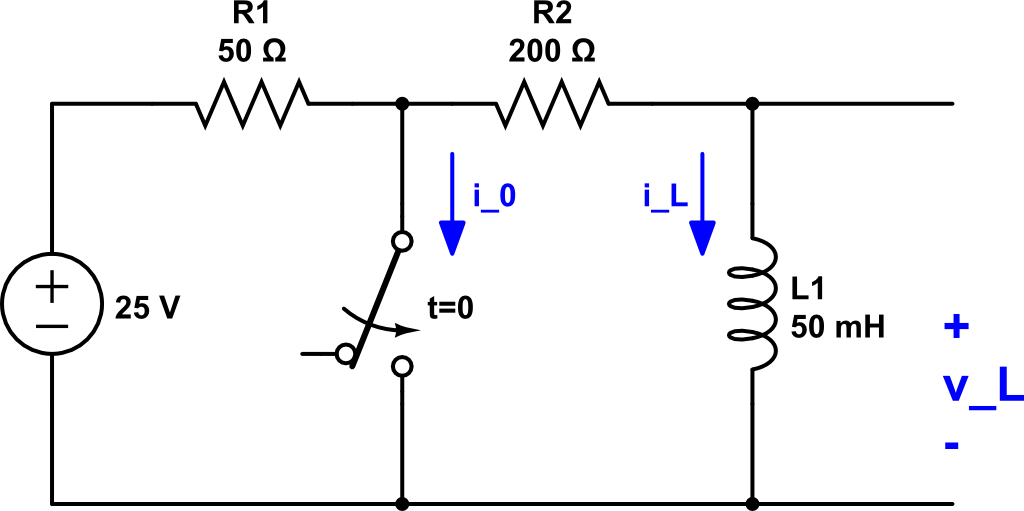
\includegraphics[scale=0.4]{p7_4.png}
\end{center}
\end{figure}

\begin{enumerate}[(a)]
\item Find $i_0(0^-)$, $i_L(0^-)$, and $v_L(0^-)$.
\item Find $i_0(0^+)$, $i_L(0^+)$, and $v_L(0^+)$.
\item Find $i_0(\infty)$, $i_L(\infty)$, and $v_L(\infty)$.
\item Write the expression for $i_L(t)$ for $t \geq 0$.
\item Write the expression for $i_0(t)$ for $t \geq 0^+$.
\item Write the expression for $v_L(t)$ for $t \geq 0^+$.
\end{enumerate}


\vspace{0.1in}


{\bf Question 2} [4] % P7-21

The switch in the circuit below has been in the left for a long time before moving right $t=0$ and staying there:

\begin{figure}[h!]
\begin{center}
 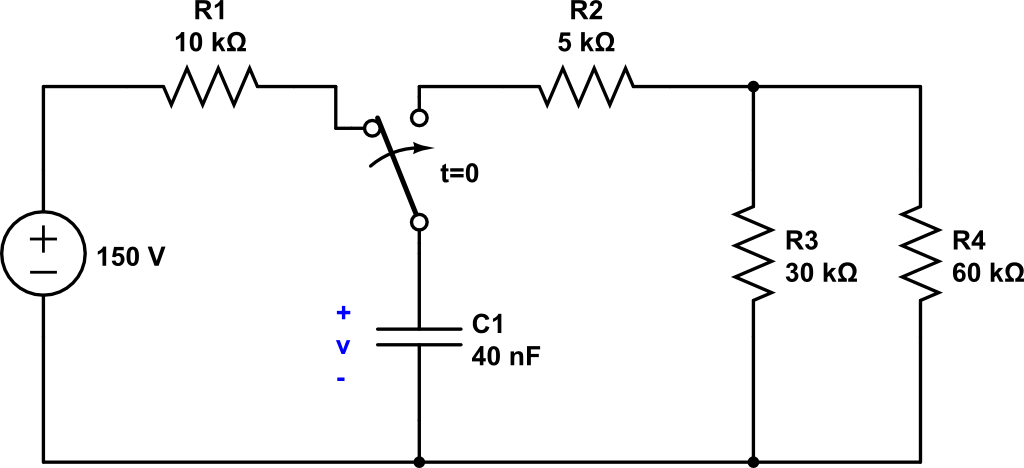
\includegraphics[scale=0.4]{p7_21.png}
\end{center}
\end{figure}

\begin{enumerate}[(a)]
\item Find the initial voltage across the capacitor.
\item Find the initial energy stored in the capacitor.
\item FInd the time constant for the circuit at $t > 0$.
\item Write the expresion for the capacitor voltage $v(t)$ for $t \geq 0$.
\end{enumerate}

\newpage

{\bf Question 3} [4] % P7-64

The switch in the circuit below has been in the left for a long time before moving right $t=0$ and staying there:

\begin{figure}[h!]
\begin{center}
 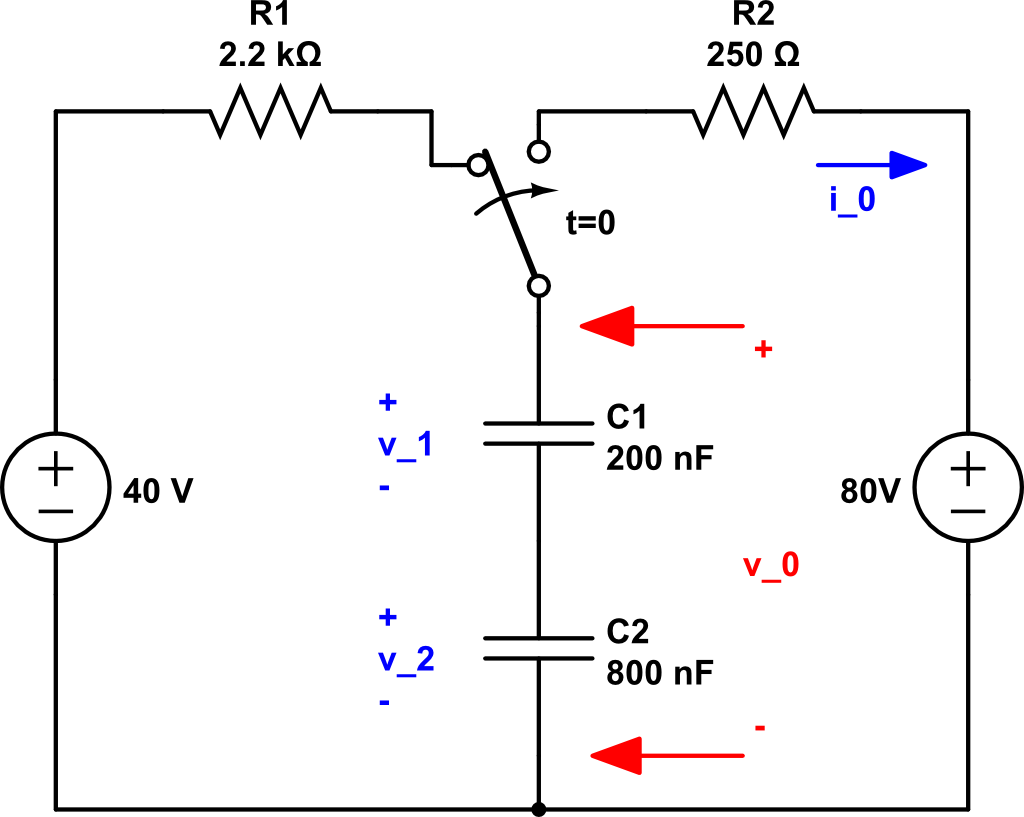
\includegraphics[scale=0.3]{p7_64.png}
\end{center}
\end{figure}

Find
\begin{enumerate}[(a)]
\item $v_0(t)$
\item $i_0(t)$
\item $v_1(t)$
\item $v_2(t)$
\item The energy trapped in the capacitors at $t \rightarrow \infty$.
\end{enumerate}



{\bf Question 4 [4]} % P7_84

The circuit below is given a $v_s$ of $50V$ from time $0ms$ to $1ms$. At $1ms$, $v_s$ is returned to zero, where it stays.

\begin{figure}[h!]
\begin{center}
 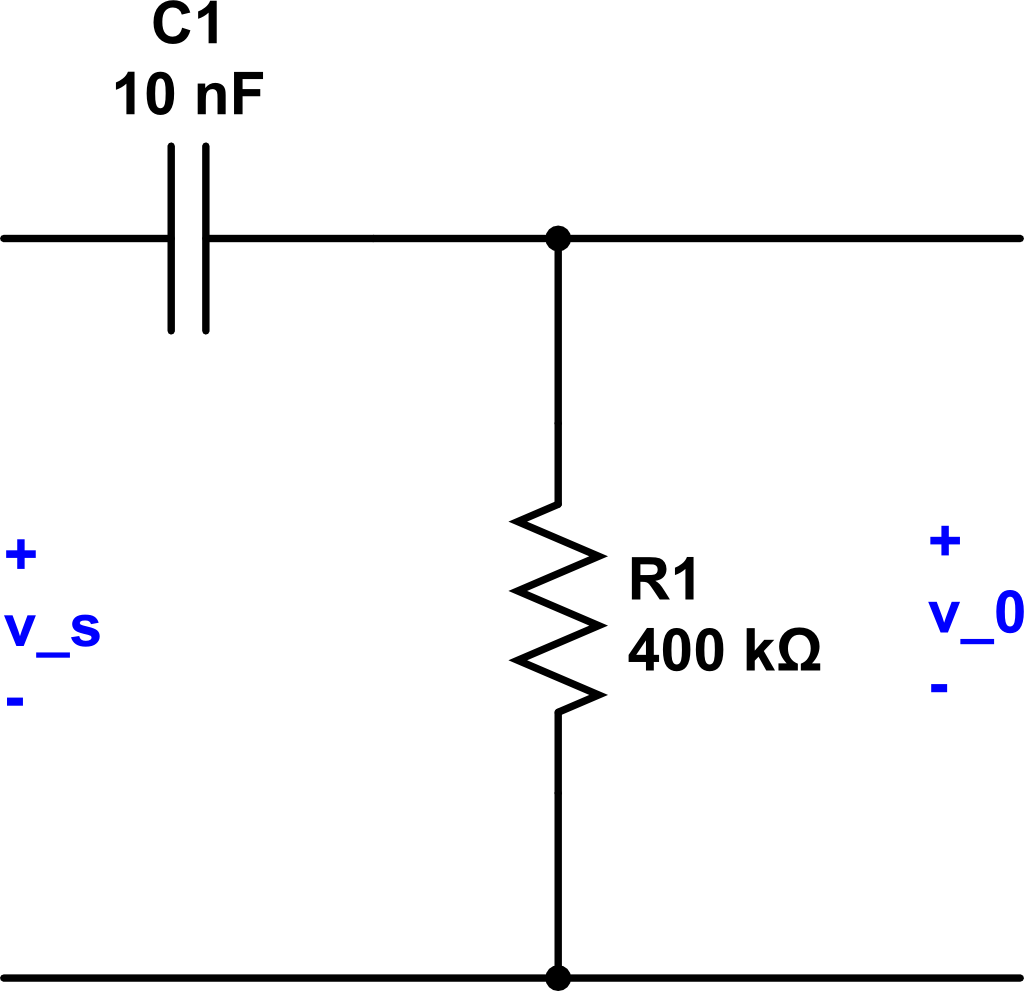
\includegraphics[scale=0.3]{p7_84.png}
\end{center}
\end{figure}

\begin{enumerate}[(a)]
\item Calculate $v_0(t)$
\item Make a sketch of $v_o(t)$ versus $t$.
\end{enumerate} 

\newpage

{\bf Question 5} [4] % P7-90

For the circuit below, the energy stored in the capacitor is zero at the instant the switch is closed. The ideal operational amplifier reaches saturation in 15ms. What is the numerical value of R?

\begin{figure}[h!]
\begin{center}
 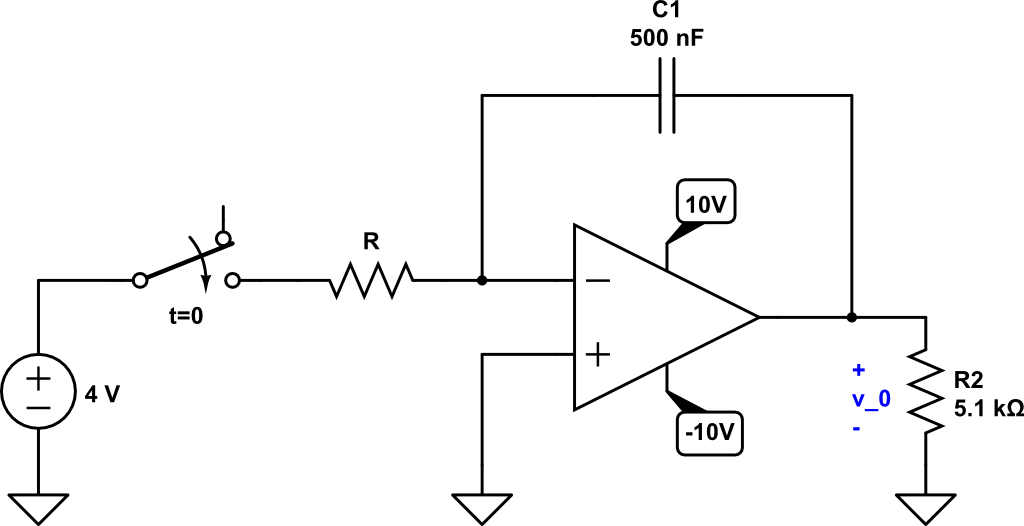
\includegraphics[scale=0.4]{p7_90.png}
\end{center}
\end{figure}

\end{document}
